\documentclass[a4paper,11pt]{article}
\usepackage[T2A]{fontenc}
\usepackage[utf8]{inputenc}
\usepackage[english, russian]{babel}

\usepackage[margin=20mm]{geometry}
\geometry{
        a4paper,
        total={165mm,247mm},
        top=30mm,
        bottom=20mm 
}

%%% Работа с картинками
\usepackage{graphicx}  % Для вставки рисунков
\graphicspath{{images/}{images2/}}  % папки с картинками

\usepackage{hyperref}
\usepackage[usenames,dvipsnames,svgnames,table,rgb]{xcolor}
\hypersetup{                            % Гиперссылки
    unicode=true,           % русские буквы в раздела PDF
    pdftitle={Заголовок},   % Заголовок
    pdfauthor={Автор},      % Автор
    pdfsubject={Тема},      % Тема
    pdfcreator={Создатель}, % Создатель
    pdfproducer={Производитель}, % Производитель
    pdfkeywords={keyword1} {key2} {key3}, % Ключевые слова
    colorlinks=true,            % false: ссылки в рамках; true: цветные ссылки
    linkcolor=red,          % внутренние ссылки
    citecolor=green,        % на библиографию
    filecolor=magenta,      % на файлы
    urlcolor=cyan           % на URL
}


\title{Установка miktex}
\author{Прокшин А.Н.} 
% Конец преамбулы
\begin{document}
\maketitle

\begin{figure}[!ht]
\centering
\caption{Заходим на сайт \href{https://miktex.org}{Mik\TeX}} 
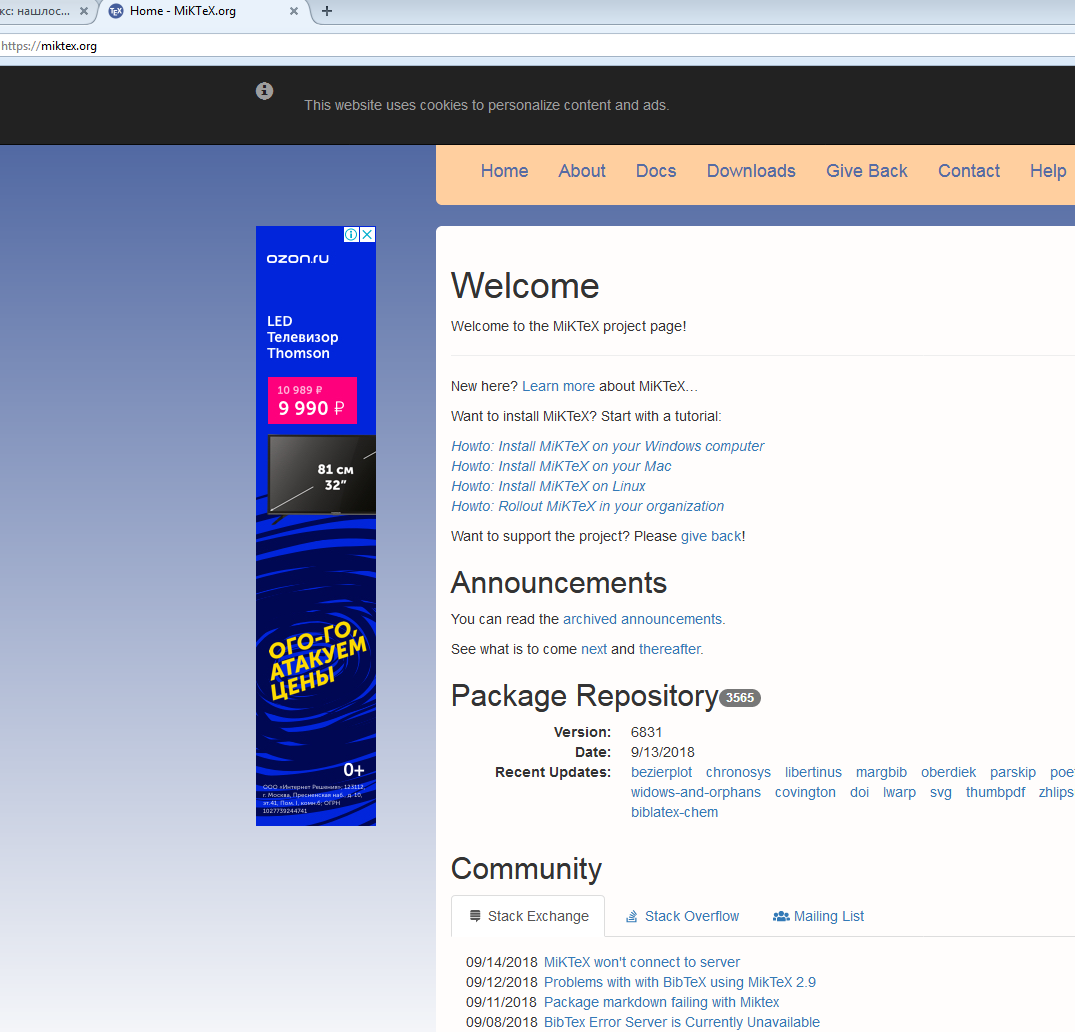
\includegraphics[width=0.48\linewidth]{miktex1.png}
\end{figure}
\begin{figure}[!ht]
\centering
\caption{Выбираем пункт меню скачивания <<Downloads>>}
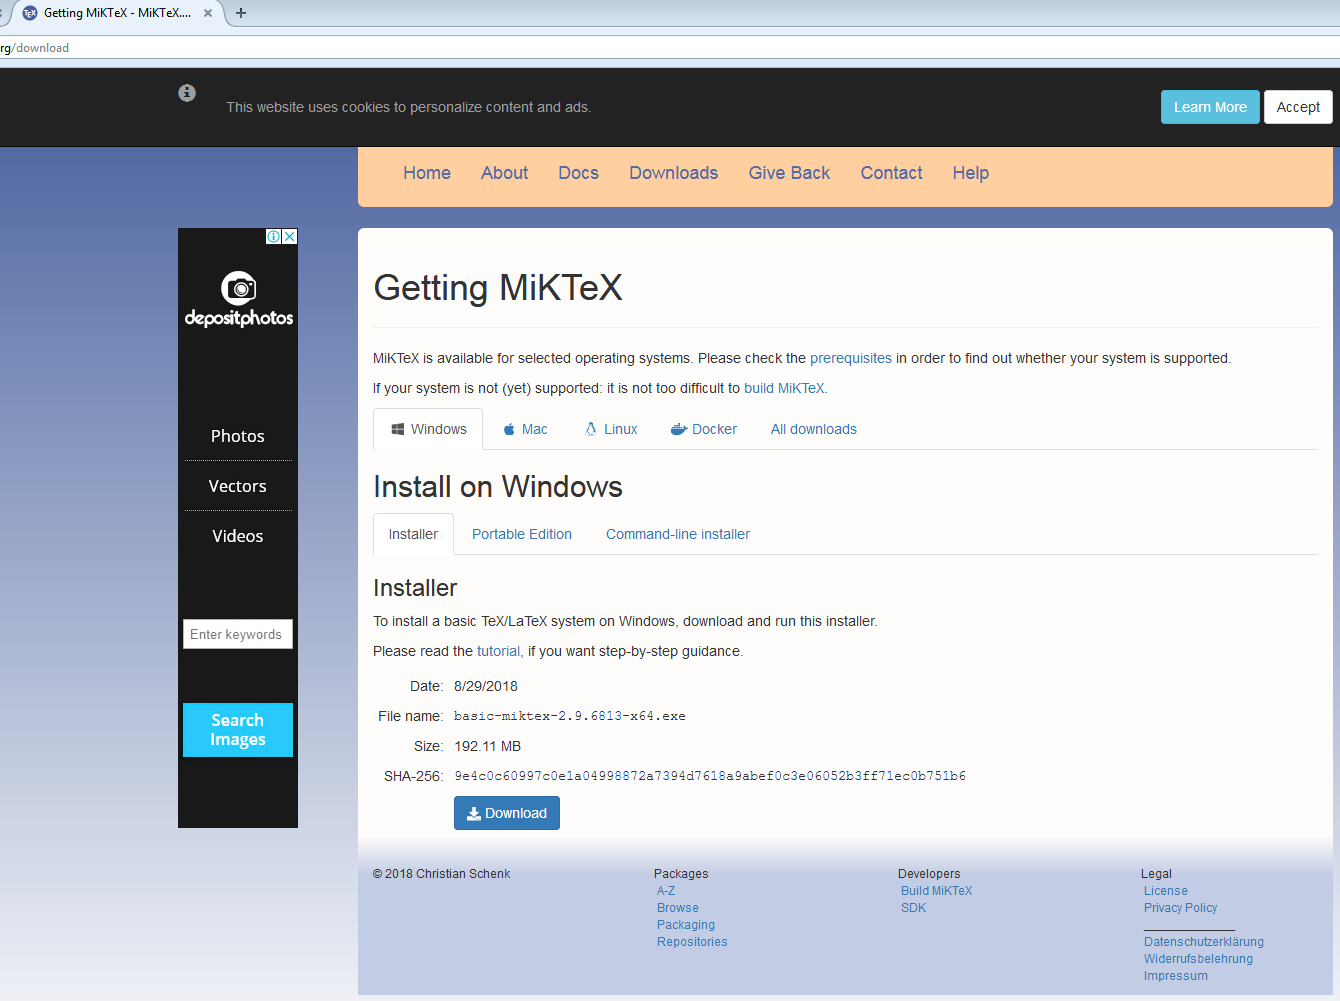
\includegraphics[width=0.48\linewidth]{miktex2.png}
\end{figure}
\begin{figure}[!ht]
\centering
\caption{загружаем \dots}
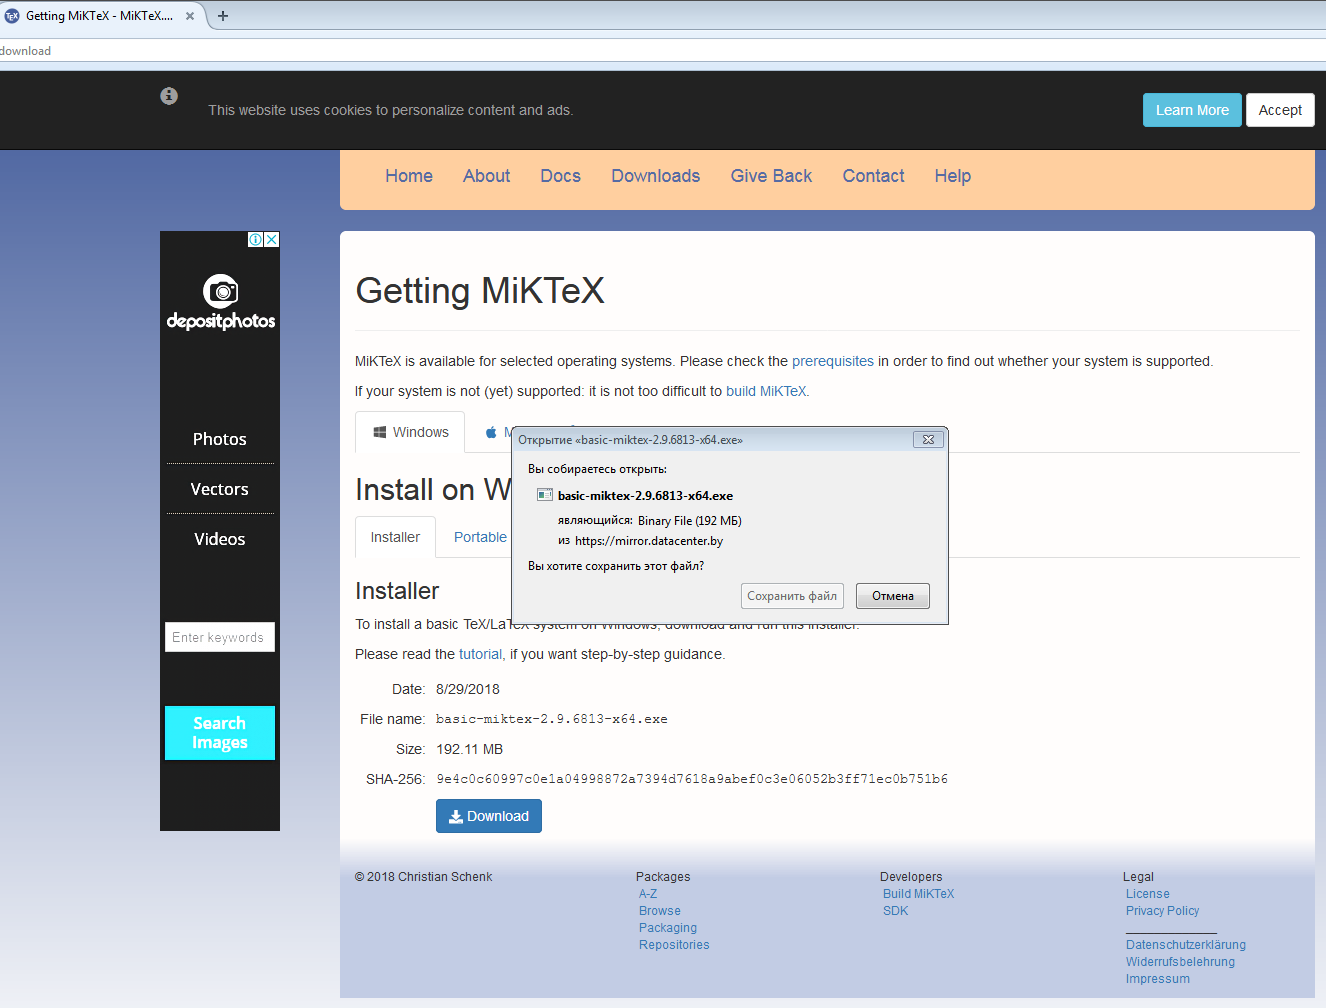
\includegraphics[width=0.48\linewidth]{miktex3.png}
\end{figure}
%Выбираем условие, как показано в \href{https://miktex.org/howto/install-miktex}{руководстве}
\begin{figure}[!ht]
\centering
\caption{Выбираем <<устанавливать только для своего пользователя>>, как показано в \href{https://miktex.org/howto/install-miktex}{руководстве}}
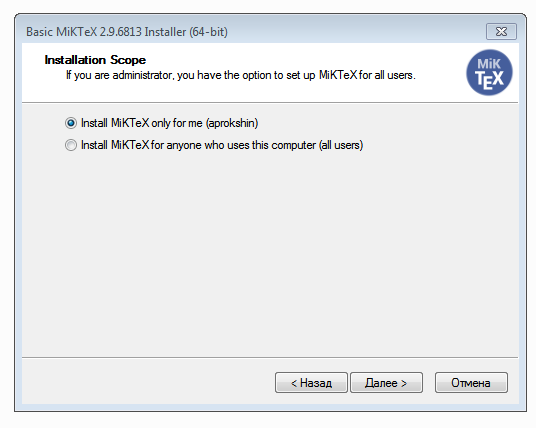
\includegraphics[width=0.48\linewidth]{miktex4.png}
\end{figure}
\begin{figure}[!ht]
\centering
\caption{Размер бумаги А4. Спрашивать меня устанавливать ли пакеты}
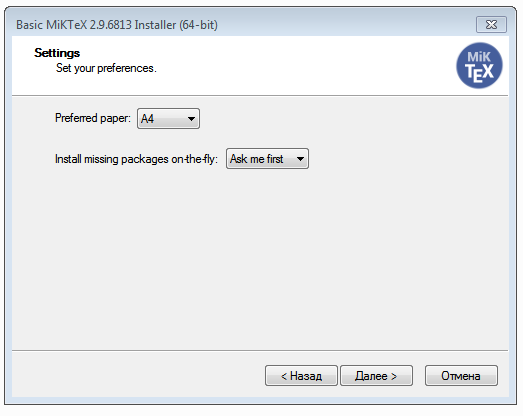
\includegraphics[width=0.48\linewidth]{miktex5.png}
\end{figure}
\begin{figure}[!ht]
\centering
\caption{Следим за процессом установки}
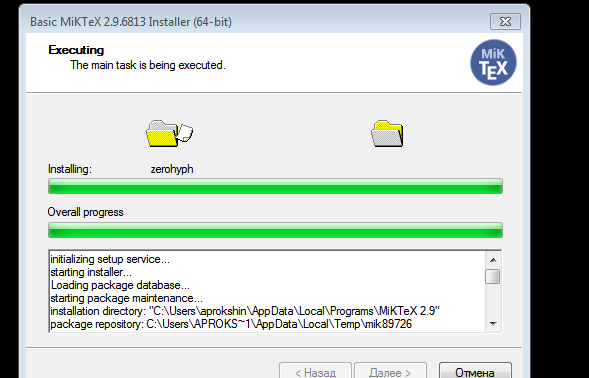
\includegraphics[width=0.48\linewidth]{miktex6.png}
\end{figure}
\begin{figure}[!ht]
\centering
\caption{Позволим обновляться}
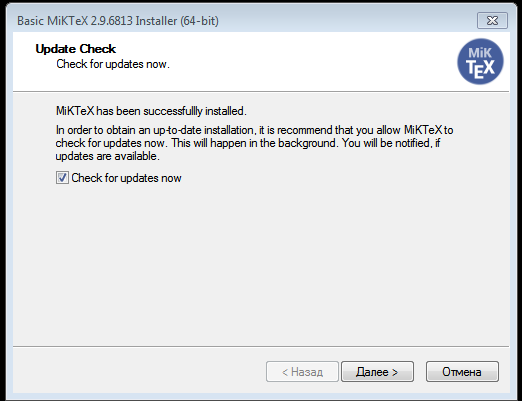
\includegraphics[width=0.48\linewidth]{miktex8.png}
\end{figure}
\begin{figure}[!ht]
\centering
\caption{После старта из ярлыка нажать на иконку с буквой T}
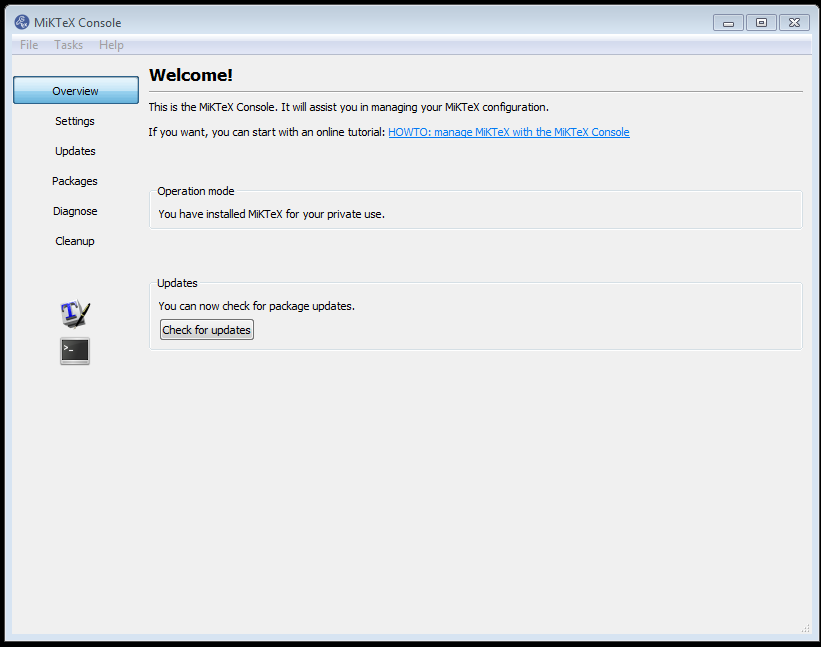
\includegraphics[width=0.48\linewidth]{miktex9.png}
\end{figure}
\begin{figure}[!ht]
\centering
\caption{Открытое окно Mik\TeX}
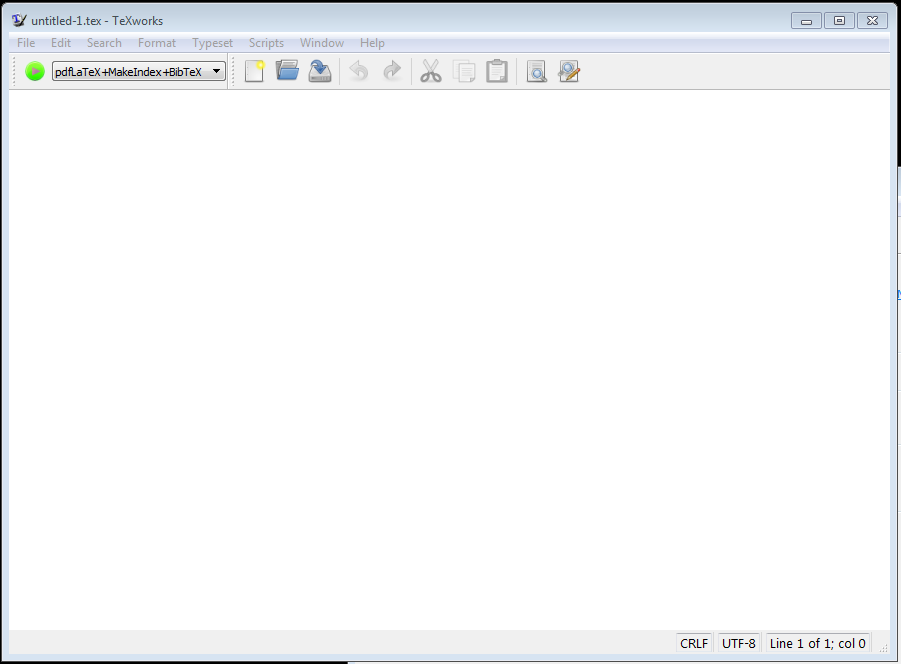
\includegraphics[width=0.48\linewidth]{miktexa.png}
\end{figure}
\begin{figure}[!ht]
\centering
\caption{При запросе об установке недостающих пакетов соглашатьься}
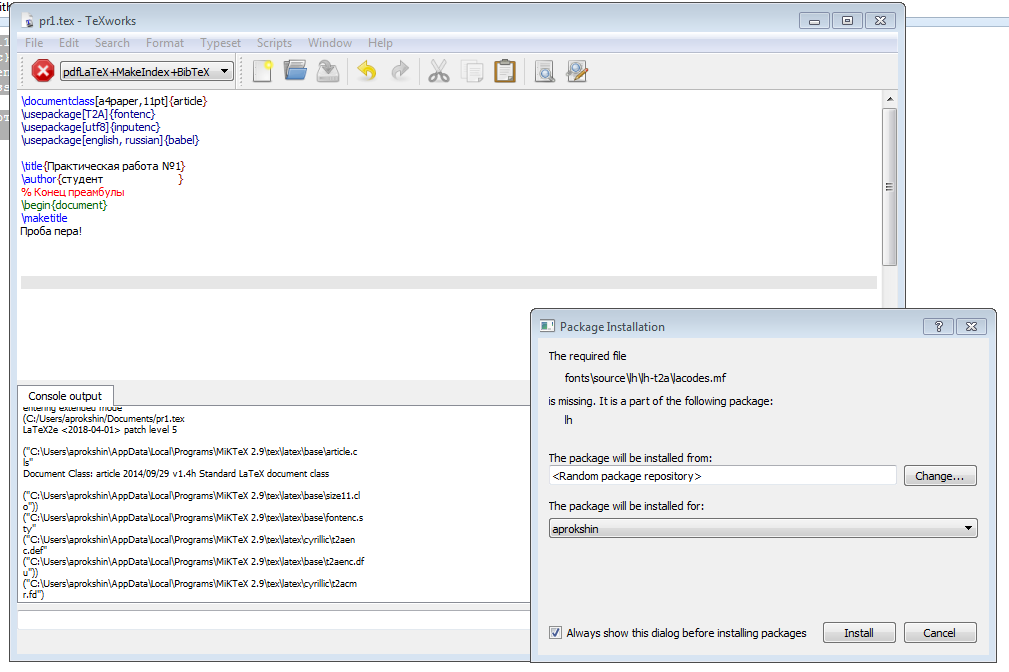
\includegraphics[width=0.48\linewidth]{miktexb.png}
\end{figure}
\begin{figure}[!ht]
\centering
\caption{Скомпилированный с помощью  Mik\TeX шаблон}
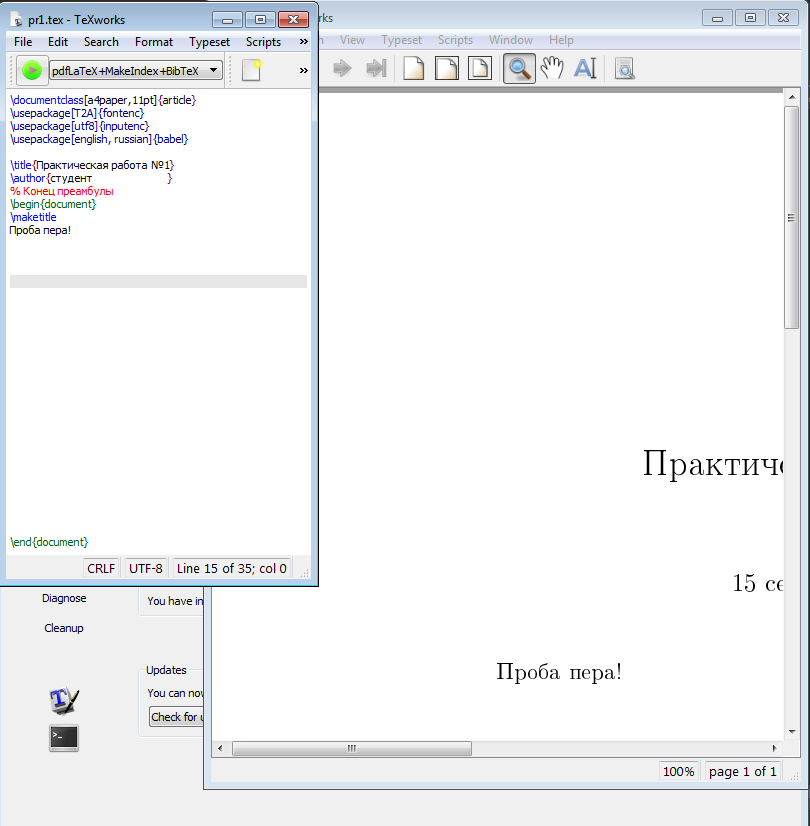
\includegraphics[width=0.48\linewidth]{miktexc.png}
\end{figure}






\end{document}
